\subsection{PINNs and Approximating Damped Harmonic Oscillators}

Finally we applied these techniques to an PINN. For our initial explorations in this space we focused on fitting to systems of damped harmonic oscillators as has been the through line of the work thus far. We chose the 3 parameter DHO embedding over the 4 parameter embedding with a pre-factor as while it was more effective when subject to direct gradient descent, we were concerned that the additional redundant embedding parameter would make learning the systems more complex and error prone. 

The dataset used ($N \approx 5 \times 10^5$) in training was a mixed selection, primarily it was comprised of uniformly distributed embeddings within the subset of the physical region of the embedding space (positive embedding values). In addition a fraction, approximately $5 \%$ for each, of the spring and damping constants were set to zero to ensure that the model was exposed to non-damped simple harmonic motion and kinetic-energy only systems.

For PINN training, accounting for the increased complexity of the optimisation problem now being with respect to the parameters of the model, we made two alterations to our loss functions. First we added a strong weight against non-physical negative embedding values in our loss function, taking the form of,

\begin{equation}
  f(e_i) = \begin{cases}
  	0 & e_i \ge \delta \\
  	\exp{-\gamma e_i} & e_i < \delta 
  \end{cases}
\end{equation}

where $\delta = −0.1$ is a tolerance to allow for zero to be a non-penalised output and $\gamma \approx 10$ is the strength of the penalisation. This was done as the non-physical behaviour of negative embedding values is less visible when considering the larger whole model optimisation problem.
In addition we also experimented with capping the values of the loss at large values to mitigate overflows when dealing with particularly bad fits, such as the initially random initialised weights before any training had commenced.

Model training was done in batches and was prone to explosion possible due to the non-convexity in some regions as discussed in \sref{sec:res-lf}. Overall it was found that training could be made more stable by increasing batch sizes to $512$ from $32$, and manually tweaking loss weightings (for example between the $\vb q$ and $\pi$ RMS terms where more progress was made with weighting towards $\vbq$ error to counteract observed larger tendency for error in this term) and learning rates as training progressed.

Other loss functions, such as RMS in $\pi$ only, were once again investigated. This produced good losses on the order of $10^{-4}$, however on further inspection it was found that these resulted from a finding a false minima of $m \approx k \approx \lambda$, highlighting the complexity of the embedding space in representing physical systems. This also underlined the utility of the previous direct embedding space optimisation done prior in informing us about the behaviour of the loss function itself.

By the training's conclusion we obtained an RMS error of $\pm 5 \times 10^{-2}$ in $\vbq$ and $\pm 1 \times 10 ^{-1}$ in $\pi$. This model was able to predict systems with some accuracy, clearly able to fit to certain features as shown in \fref{fig:model-prediction}.

\begin{figure}[t]
  \label{fig:model-prediction}
  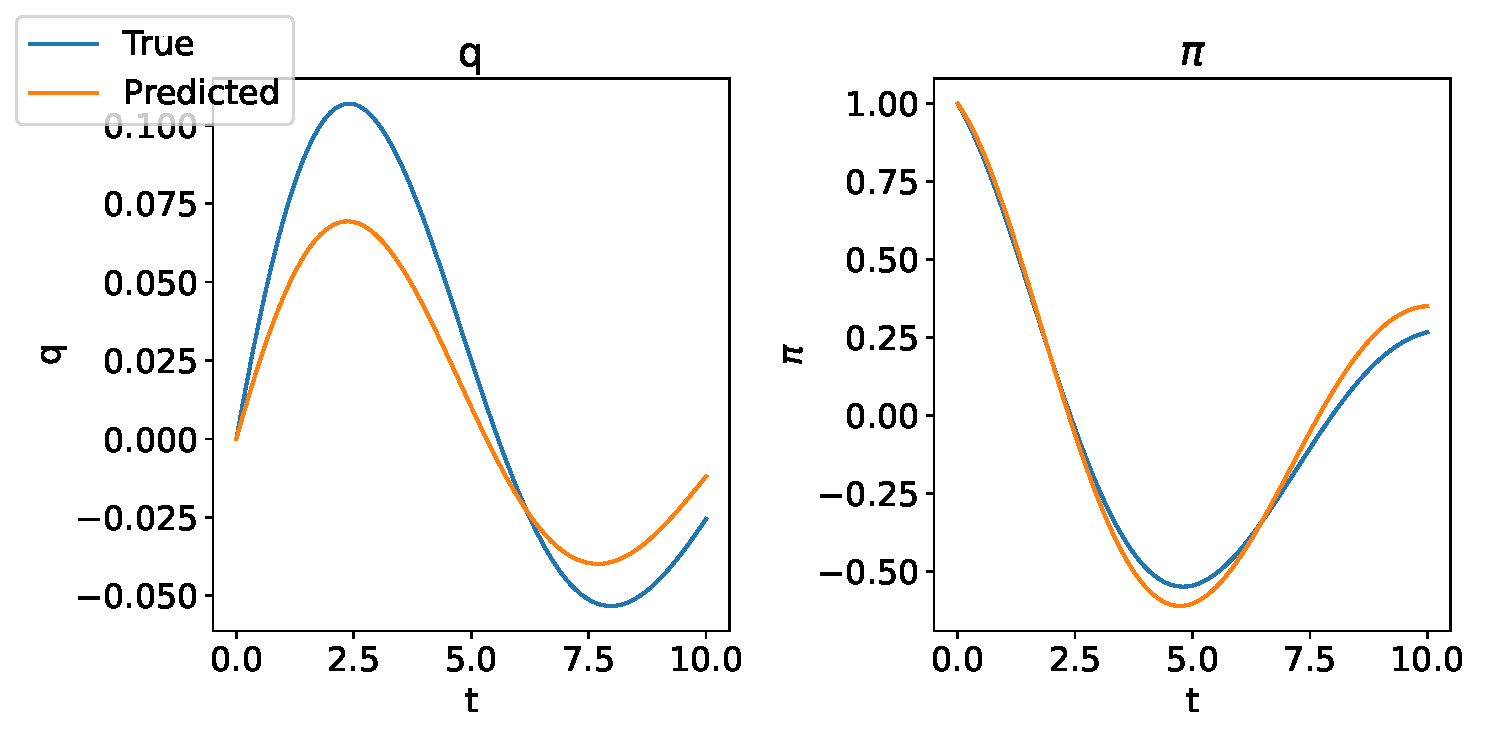
\includegraphics[width=\columnwidth]{figures/model-predictions.pdf}
  \caption{A comparison of the behaviour of a Lagrangian embedding predicted by a PINN. True embedding, $(m = 6, k = 2, \lambda = 3)$, predicted embedding, $(m = 9.401553,  k = 3.3729377, \lambda = 3.9162085)$.}
\end{figure}

